%\documentclass[prodmode]{acmsmall-ec16}
%\documentclass[prodmode,license]{acmsmall-ec16}
\documentclass[prodmode,permissions]{acmsmall-ec16}

% Package to generate and customize Algorithm as per ACM style
\usepackage[ruled]{algorithm2e}
\renewcommand{\algorithmcfname}{ALGORITHM}
\usepackage{amsmath,amsfonts,amssymb,bbm} 
\usepackage[numbers,sort&compress]{natbib} % for citet
\SetArgSty{textrm}  % for algorithm2e
\SetAlFnt{\small}
\SetAlCapFnt{\small}
\SetAlCapNameFnt{\small}
\SetAlCapHSkip{0pt}
\IncMargin{-\parindent}

%\conferenceinfo{EC'16,}{July 24--28, 2016, Maastricht, The Netherlands.}
%\CopyrightYear{2016}
%\crdata{978-1-4503-3936-0/16/07}
%\copyrighttext{Copyright is held by the owner/author(s). Publication rights licensed to ACM.}

\doi{XXXXXXX.XXXXXXX}% TeXSupport

\usepackage{tikz}
\usetikzlibrary{arrows,chains,decorations.pathreplacing}
\newcommand{\beq}{\begin{eqnarray}}
\newcommand{\eeq}{\end{eqnarray}}
\DeclareMathOperator{\wbf}{wBF}

% Document starts
\begin{document}

% Page heads
%\markboth{G. Zhou et al.}{A Multifrequency MAC Specially Designed for WSN Applications}

% Title portion
\title{
Attack-Tolerance in Structured Networks via Multipath Routing
\\ Draft: 2016-02-21
}
\author{EDWARD L. PLATT
\affil{University of Michigan}
DANIEL M. ROMERO
\affil{University of Michigan}}

\begin{abstract}
TODO
\end{abstract}

%ACM is moving forward with the 2012 Classification system: http://dl.acm.org/ccs_flat.cfm. Please generate the CCSXML tex code through the online interactive system and insert the code below. 

\begin{CCSXML}
<ccs2012>
</ccs2012>  
\end{CCSXML}

\ccsdesc[500]{TODO~TODO}

%\terms{Design, Algorithms, Performance}

\keywords{
censorship,
decentralization,
fault tolerance,
multipath,
networks,
peer-to-peer,
trust
}

\begin{bottomstuff}
This work is supported by TODO.

Author's addresses: E.L. Platt and D.M. Romero, School of Information; email: \{elplatt,drom\}@umich.edu.
\end{bottomstuff}

\maketitle

TODO:\\
Fix bibtex encoding\\
Move secrecy section\\
Add ref to unipath butterfly routing\\
Update intro to make significance more clear\\

\section{Introduction}

Large-scale communication networks, exemplified by the Internet,
have become ubiquitous and critical infrastructural for
communities, organizations, and markets.
As with any critical infrastructure, the cost of a failure can be
immense, so methods for tolerating various kind of faults are an
important and ongoing area of research
\cite{zin_survey_2015,albert_error_2000,sterbenz_resilience_2010}.
The key question is: what are the techniques and network structures that can
be used to create robust, fault-tolerant systems?

Many complex networks, including the Internet and World-Wide Web, exhibit
scale-free structure
\cite{barabasi_emergence_1999,barabasi_scale-free_2009}.
While scale-free networks tolerate random faults well,
they are highly susceptible to adversarial faults, i.e. attacks
\cite{albert_error_2000}.
For example, in 2008, YouTube suffered a worldwide outage for several hours
when a service provider in Pakistan advertised false routing information
\cite{hunter_pakistan_2008}.
The action (known as a {\em black hole attack}) was intended to censor YouTube
within Pakistan only, but resulted in a worldwide cascading failure.
Such vulnerabilities are not limited to any one system or protocol, but an
attribute of complex communication networks themselves.
General techniques for understanding and mitigating these vulnerabilities are
needed.

We consider a setting in which a source node in a network attempts to route information
to a target node by forwarding it through the links of the network. We 
assume that some nodes in the network may be compromised by an attacker 
and will forward the wrong information to their neighbors or
block the information altogether.
In order to evaluate network-based techniques for mitigating such attacks,
we develop a decentralized {\em partial trust} model,
similar to a web of trust
\cite{zimmermann_official_1995,ferguson_practical_2003},
but making weaker assumptions of trust transitivity.

Given this framework, we develop and evaluate a \emph{multipath routing} technique to reduce 
the likelihood that compromised nodes are undetected during the information 
routing process by allowing multiple copies of a message to be sent through independent paths,
which can be used for error-detection and error-correction by the receiver. 

The multipath routing technique relies on the existence and discoverability of
multiple redundant paths between the source and the destination. Thus, network 
structure and routing algorithms play a key role in the success of the technique.
We formally evaluate the 
effects of network structure on attack-resistance and show that the probability
of undetected 
errors decreases exponentially with the number of independent paths between 
source and destination.

The mutlipath routing technique is well-suted for {\em structured networks},
in which links between nodes are constrained to a particular architecture.
Specifically, we employ the butterfly network topology,
used elsewhere in parallel computing \cite{kshemkalyani_distributed_2008}
and peer-to-peer \cite{lua_survey_2005, korzun_structured_2013}
applications.
For this network topology,
we propose an efficient, attack-tolerant multipath routing algorithm.

Our main contributions are:
\begin{itemize}
\item{We develop a decentralized {\em partial trust model},
which makes weaker transitivity assumptions than previous web-of-trust models,
and use this model to quantify the effects of network structure on
fault tolerance;}
\item{We show that as the number of disjoint paths between the neighborhoods
of the sender and reciever grows,
the probability of successfully detecting adversarial faults
approaches 1 exponentially.
Furthermore, we show that the number of disjoint paths is a function of
network structure;}
\item{We present a scalable, efficient, and attack-tolerant multipath
routing algorithm on the butterfly network topology.}
\end{itemize}

Paper organization. TODO

\section{Background and Related Work}

In {\em structured networks}, link structure is predetermined.
Such networks can be designed to have favorable structural and routing properties,
at the expense of complicating the addition or removal of nodes.
Structured networks have been a popular tool in parallel and distributed
computing architectures \cite{kshemkalyani_distributed_2008}.
More recently, peer-to-peer systems based on distributed hash tables have used
structured ``overlay'' networks to map table keys to local TCP/IP routes
\cite{lua_survey_2005,korzun_structured_2013}.

Many distributed consensus protocols (such as those used by crypto-currencies)
are designed to provide tolerance against arbitrary or adversarial faults.
Byzantine agreement protocols
\cite{lamport_byzantine_1982,castro_practical_1999}
provide tolerance against arbitrary faults (including attacks) under
some circumstances, but are limited to small networks due to poor scalability.
Proof-of-work \cite{dwork_pricing_1993,nakamoto_bitcoin:_2008}
and proof-of-stake \cite{king_ppcoin:_2012}
provide better scalability, but wasteful of computational and energy
resources.
Federated Byzantine Agreement (FBA) \cite{mazieres_stellar_2015}
is scalable and optimal, guaranteeing that the protocol only fails when
success is impossible, although it does not provide a way to evaluate
the probability of failure.
All of these protocols rely on the assumption that their cryptography
cannot be compromised.
While cryptography can be extremely resistant to technological attacks,
it can still be compromised through coercion (e.g., legal action).
In additon, the fault-tolerance of FBA depends on redundancy in the network structure
but leaves an unanswerd question: how should a network be structured to achieve
fault tolerance?
This paper addresses both of these issues by analyzing the role of network
structure on adversarial faults, without relying on assumptions of cryptographic
integrity.

{\em Multipath} routing uses multiple paths when routing a message through a
network, in contrsast to traditional {\em unipath} routing, which uses
a single path.
Multipath routing can have many benefits, including reduced congestion,
increased throughput, and more reliability
\cite{qadir_exploiting_2015}.
Many of these routing protocols offer better security 
\cite{zin_survey_2015}.
Some approaches utilize redundant paths as backups for increased
fault tolerance
\cite{alrajeh_secure_2013},
and some specificially protect against adversarial faults
\cite{kohno_improvement_2012, khalil_unmask:_2010, lou_h-spread:_2006}.
The method of Liu et al.
\cite{liu_secure_2012}
routes multiple messages first to random peers and then
to their final destination.
The butterfly algorithm we present takes a conceptually similar approach.
Most work on multipath routing has been motivated by applications related to
wireless sensor networks (WSNs),
and have thus focused on ad-hoc, unstructured networks, often having a central
base station.
The trust model presented in this paper provides a more general way to evaluate
the effect of network structure on adversarial fault-tolerance.

\section{Attack-Tolerant Networks Infrastructure}

In this section, we describe the functional properties required of an
attack-tolerant network infrastructure and how those properties translate
into constraints on network structure.
We pay special attention to a property we call
{\em stabilizing asymmetry}.

\subsection{Functional Properties}

\begin{description}
\item[Scalability]
For large scale networks it is important that the infrastructure allows for the network to grow while remaining functional. In practice, people, devises, and connections, have limited capabilities and these limitations need to be considered as part of the design of the infrastructure. 

\item [Decentralization]
Systems having single points of failure are less tolerant against faults at those
points, which both raises the likelihood of a failure and creates targets
where attackers might be able to focus their resources efficiently.
Attack-tolerant infrastructure must be decentralized in order to minimize single points of failure.

\item[Stabilizing asymmetry]
In the context of international conflict,
\cite{mack_why_1975}
observed that power imbalance usually determines the outcome of a conflict
(with the more powerful side winning)
except in the special case of {\em asymmetric conflicts}.
In asymmetric conflicts, the same level of resource expenditure yields different
results for different parties.
There are two possible cases:
the attacker's resources are either more or less effective than the defender's.
We call the latter case stabilizing asymmetry,
because it lowers the incentive to attack.
With this in mind, an attack-resistant infrastructure will benefit from a high
level of stabilizing asymmetry.

\item[Secrecy]
In some, but not all cases, it is desirable that the infrastructure provides secrecy and allow a source and a target to exchange private information while still relying on intermediary nodes. Our proposed multipath routing technique can be adapted to provide secrecy but we do not focus on this aspect in this paper. 

\end{description}
\subsection{Structural Properties}

We now describe the structural properties of a network that allow it to achieve the functional properties described above. 
\begin{description}
\item [Sparsity and low diameter]
To achieve scalability, networks must be {\em sparse} and have a
{\em low diameter}.
In practical settings, humans and devices have an upper limit on the number
of connections they can maintain.
In sparse networks, the number of links grows slowly as the network grows in
size, allowing the network to scale without exceeding the nodes' capacity for
links.
Similarly, low-diameter guarantees that as a network grows, a short path will
still exist between any pair of nodes.
While low diameter guarantees a path exists,
paths are only useful if an efficient {\em routing} algorithm exists
to find them.

\item [Vertex transitivity]
In vertex transitive networks, for any pair of nodes, an edge-preserving map
always exists from one node to the other.
In other words, all nodes occupy structurally indistinguishable positions
in the network. Networks with {\em vertex transitivity} are decentralized in the sense that they structure does no allow for  single points of failure.

\item [Redundancy]
Redundancy in a network refers to the extent to which nodes are connected to each other by multiple independent paths. Redundancy can help reduce single points of failure as well as
increase fault-tolerance.
One measure of redundancy is given by the ratio of edges to nodes
\cite{baran_distributed_1964}.
A single point of failure occurs when a node holds a uniquely
central position,
and can be eliminated by adding alternative
paths around the node,
which increases the network's redundancy.
Similarly, as we will later show, redundancy in a network can enable fault-tolerance techniques
that reduce the effectiveness of attacks and creating stabilizing asymmetry.
When secrecy is desired, redundancy can help by allowing messages to be
divided into parts and sent along different paths so even if one path is
compromised, the whole message is not revealed \cite{}. 

\end{description}

\subsection{Trust}

The sparsity requirement has an important consequence for network infrastructure:
as a network grows, the number of nodes will exceed the number of links a given
node can support and many pairs of nodes will only be indirectly connected,
with all paths between them passing through at least one intermediary node.
These intermediary nodes are targets for potential attacks.
More specifically, the threat model is as follows: Alice sends a message to
Bob via one or more intermediaries, but some intermediaries may try to
either block or alter the message.
The ability to tolerate these types of adversarial attacks depends on
Alice and Bob's ability to assume that some nodes have not been
compromised---to {\em trust} them.

Both centralized and decentralized approaches are commonly used to create
trust infrastructures.
Centralized approaches such as {\em public key infrastructure} (PKI)
suffer from a number of vulnerabilities
\cite{ellison_ten_2000},
which stem largely from the single points of failure inherent to
centralization.
Alternatively, the decentralized {\em web of trust} model
\cite{zimmermann_official_1995,ferguson_practical_2003}
allows individuals
to choose who they trust initially.
Trust is then extended to new individuals if they are vouched for by a
currently-trusted individual.
However, the web of trust approach assumes that trust can be extended
transitively,
which is not generally true
\cite{christianson_why_1997}.
We note that while such approaches are decentralized in the sense that no central authority holds the keys,
they do not necessarily incorporate redundancy and the network they form may not be vertex transitive. Thus they still may suffer from single
points of failure.

\section{Partial Trust}

We now propose a decentralized trust model based on weaker transitivity
assumptions than existing web of trust models.
In following sections, we will use this model along with network redundancy to minimize vulnerabilities due to single points of failure.
Our model is based on the assumption of partially-transitive trust.
While this assumption is still idealized, it is a more realistic improvement
on fully-transitive models.

Our model (Figure \ref{fig:trust-source})
is represented as an undirected graph,
with nodes representing individual
agents and edges representing mutual trust relationships.
We define a {\em trust radius} $h$ and assume that trust is transitive
up to $h$ hops away.
In other words, the nodes $v$ and $w$ trust each other if the distance between $v$ and $w$, $d(u,v)$ is less than $h$.
For a given node $v$, we call the set of nodes that $v$ trusts the {\em trusted neighborhood} $T_h(v)$,
and all nodes at exactly distance $h$ from $v$ the {\em trust boundary} $B_h(v)$:
\beq
T_h(v) &=& \left\{ w \mid d(v,w) < h \right\} \\
B_h(v) &=& \left\{ w \mid d(v,w) = h \right\}.
\eeq
We assume that $v$ is very familiar with nodes in its trusted neighbor and $v$ would know if any of these nodes were compromised by an attacher. Hence, an adversary of $v$ has no incentive to compromise a node in  $T_h(v)$. We thus assume that no nodes within the trusted neighborhood are compromised
by an adversary of $v$. However, by compromising all nodes in the trust boundary, an adversary can
ensure that all communications leaving the trusted neighborhood are compromised. 

\begin{figure}
\centerline{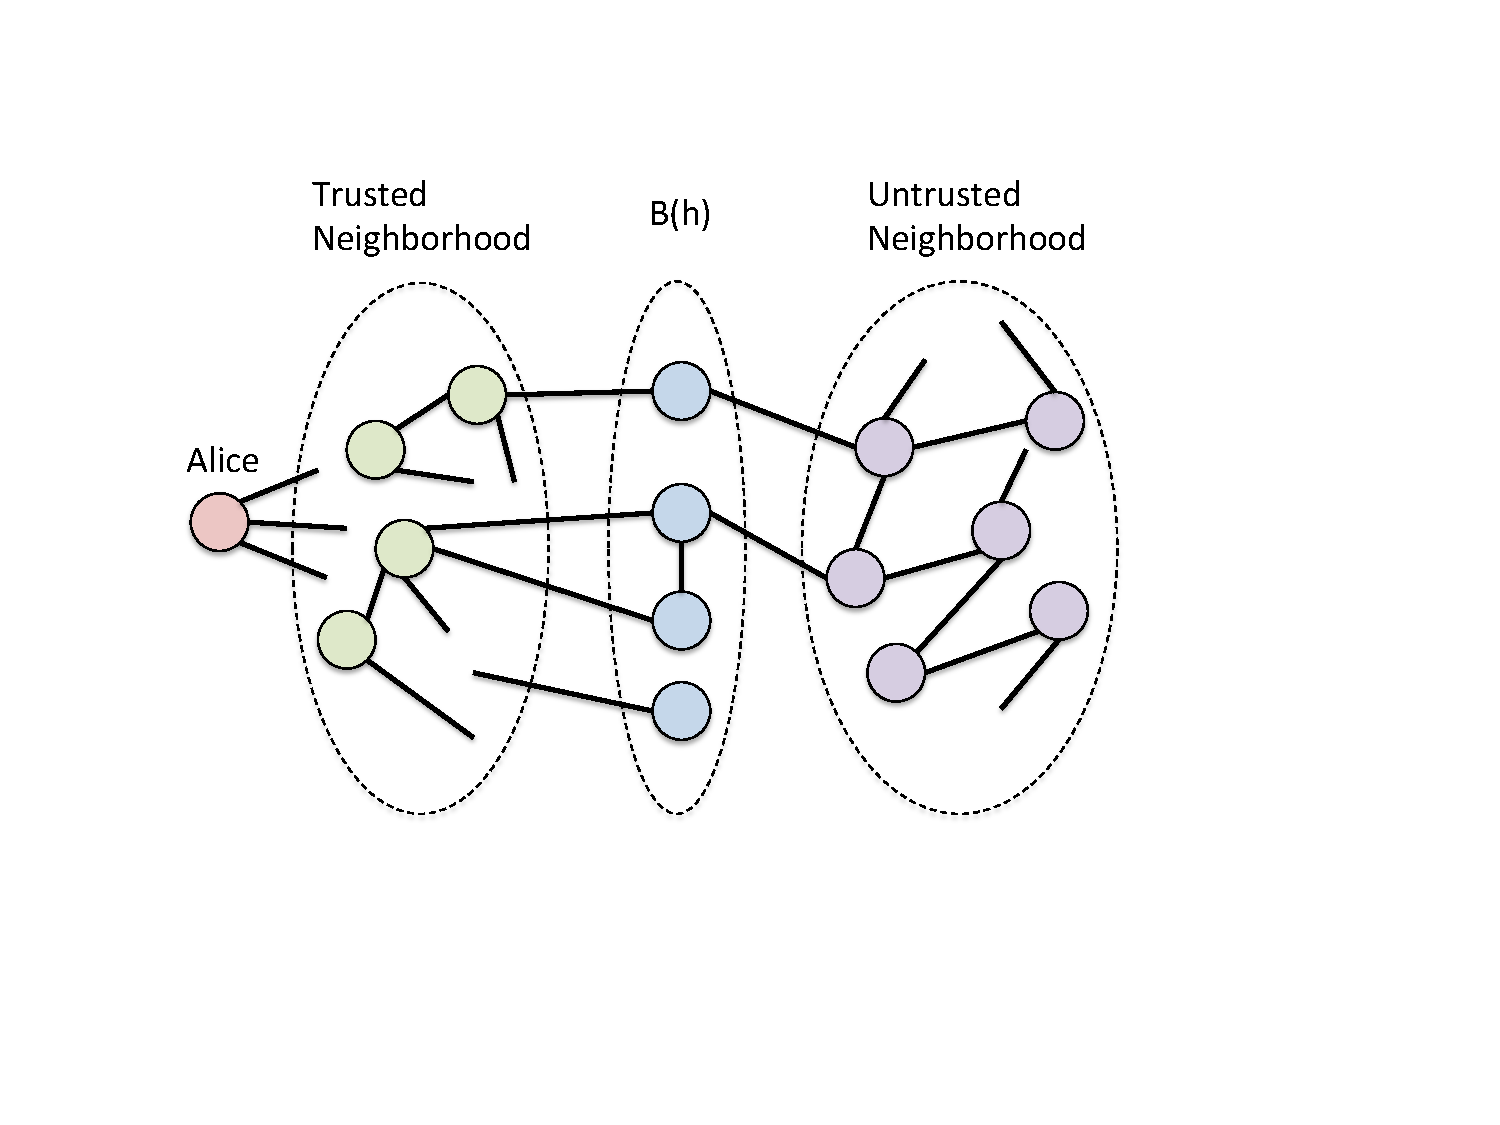
\includegraphics[height =.4 \textwidth]{fig-alice_trusted_neigh2}}
\caption{
Illustration of the {\em partial trust} model.
Edges represent direct, mutual trust relationships.
Alice ($v$) trusts all nodes less than
$h$ hops away---her {\em trusted neighborhood} $T_h(v)$.
Beyond that, the nodes at distance $h$ form her {\em trust boundary} $B_h(v)$.
We assume adversaries are unable to compromise nodes in the trusted neighborhood.
By compromising all nodes in the trust boundary, an adversary can ensure that
all communications leaving Alice's trusted neighborhood are compromised.
}
\label{fig:trust-source}
\end{figure}

Now we consider a source $v$ (Alice) and a destination $w$ (Bob),
shown in Figure \ref{fig:trust-source-destionation}. We also consider an adversary who aims at disrupting all possible communication paths between Alice and Bob. Since the adversary cannot compromise any nodes in the trusted neighborhoods of Alicia or Bob, the only option is to compromise nodes outside of the trust neighborhoods. An adversary could, for example, compromise all possible paths between Alice and Bob by compromising either Alice or Bob's entire trust boundary. This would require compromising $\min(|T_h(v)|, |T_h(w)|)$ nodes. In a vertex transitive network, these two trust boundaries will be the same size. Alternatively, the adversary could try to compromise a small set of nodes such that all paths between Alice and Bob pass through one of these nodes. However, If disjoint paths exist connecting each node in Alice's trust boundary to
a node in Bob's, then the cut size between the two can never be smaller than
$|T_h(v)| = |T_h(v)|$, so an adversary who compromises fewer nodes cannot compromise all possible paths between Alice and Bob.

\begin{figure}
\centerline{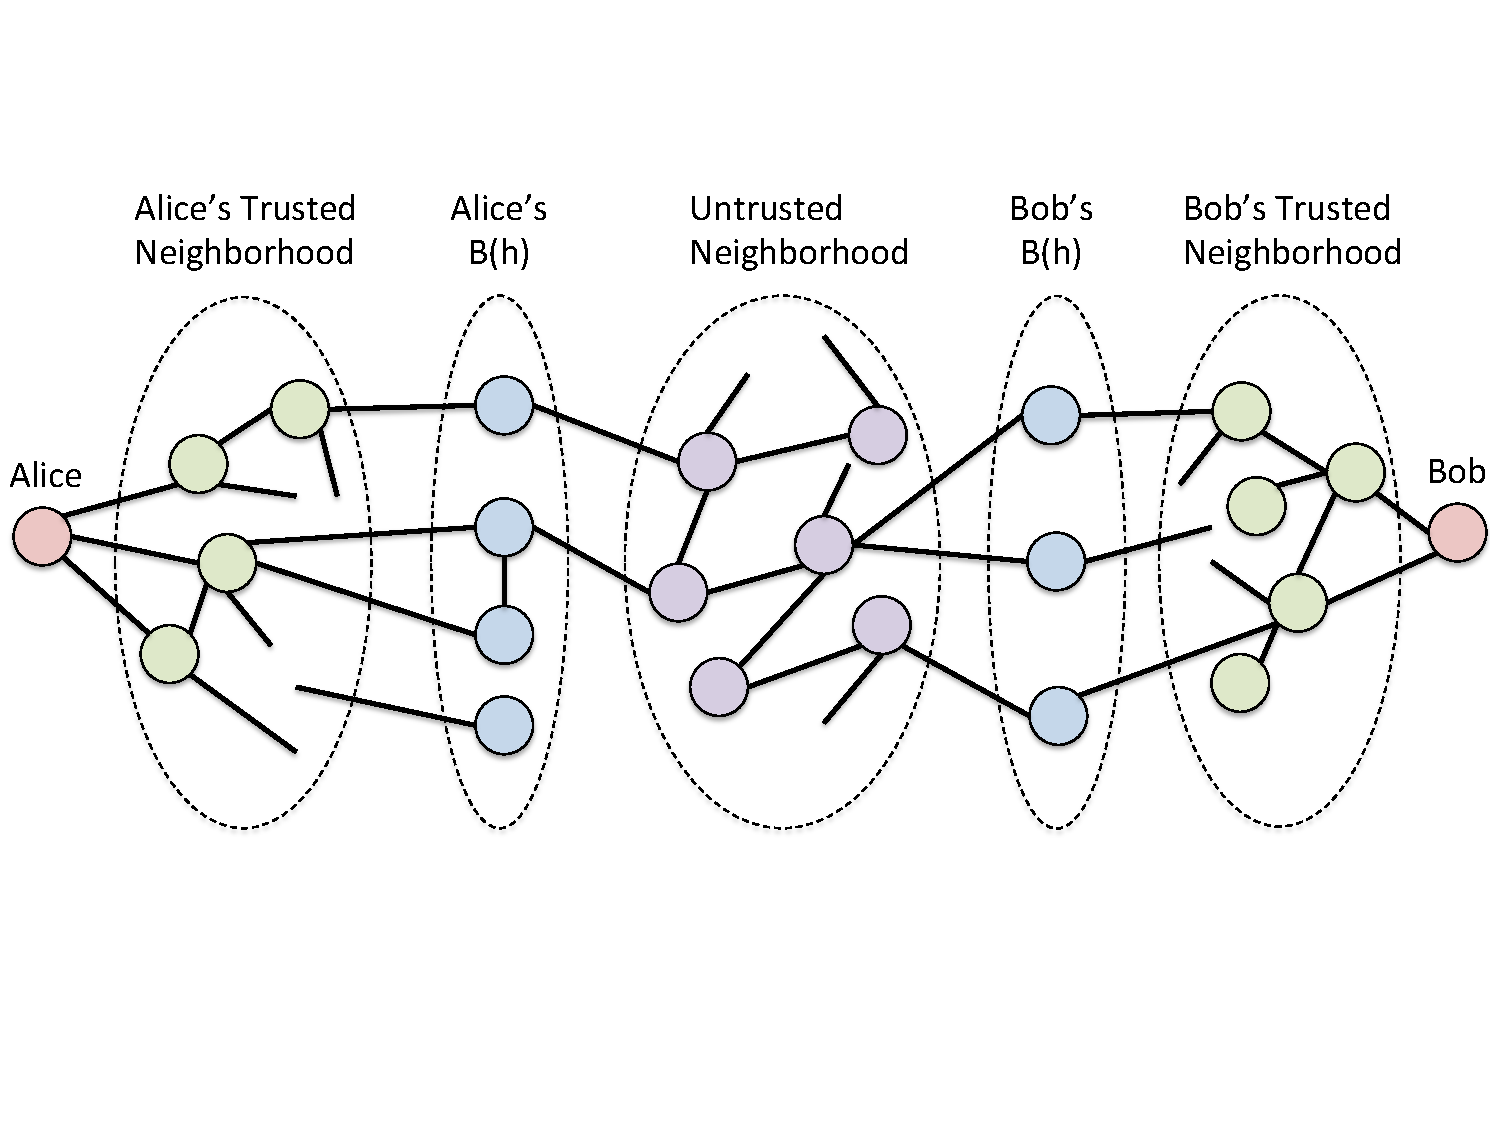
\includegraphics[height =.4 \textwidth]{fig-bob_Alice_trusted_neigh2}}
\caption{
Partial trust model with sender (Alice) and receiver (Bob).
If disjoint paths exist connecting each node in Alice's trust boundary to
a node in Bob's,
than an adversary needs to compromise at least $|T_h(v)|$ nodes to
compromise all possible paths between Alice and Bob.
}
\label{fig:trust-source-destionation}
\end{figure}

\section{Multipath Fault Tolerance}

When the assumptions of the partial trust model hold, a network can achieve
robust fault tolerance by utilizing the redundancy of multiple paths
between the sender and receiver.
Furthermore, this fault tolerance can remain robust even when faults are
adversarially chosen by an attacker who has access to more resources
than the sender and receiver.
On a structured network, multipath fault tolerance reveals not just when
an error has occured, but also which routes are faulty and potentially
compromised.

In the terminology of fault tolerance, a {\em fault} occurs when one component
of a system behaves incorrectly (e.g., a routing node blocking or
altering a message).
The result of that fault (e.g., a recipient receiving conflicting messages)
is an {\em error} state.
If the error is undetected or incorrectly corrected, the system is
said to have experienced a {\em failure} (e.g., an altered message is
accepted as authentic).
We are concerned in particular with {\em adversarial faults},
which (as opposed to random faults)
are chosen strategically (within the assumptions of the trust model)
to maximize the liklihood of a failure.
In this section, we focus on the simplest possible question:
when using multipath fault tolerance,
what is the probability that adversarial faults will cauase an undetectable
error, and thus guarantee a failure?

They key idea behind multipath fault tolerance is that several copies of
a message are sent, along multiple routes,
rather than using traditional unicast routing.
If any of the message copies differ from one another or do not arrive,
the receiver can conclude that an error has occurred,
and possibly correct it, depending on the magnitude of the error
and the desired fault tolerance properties.
In the simplest such scheme, a sender broadcasts copies of a message
along all possible routes to the receiver.
Such an approach takes advantage of all possible redundancy in the network,
and requires an adversary to compromise at least one node on each path
in order to create an undetectable error.
Realistically, the sender may only have the resources to send a limited number of
copies, or the network may not be able to handle the congestion caused by
sending all messages along all paths.
However, we will now show that a network can provide a high level of
fault tolerance with only a few copies of a message,
provided the number of possible paths is large.

\begin{figure}
\centerline{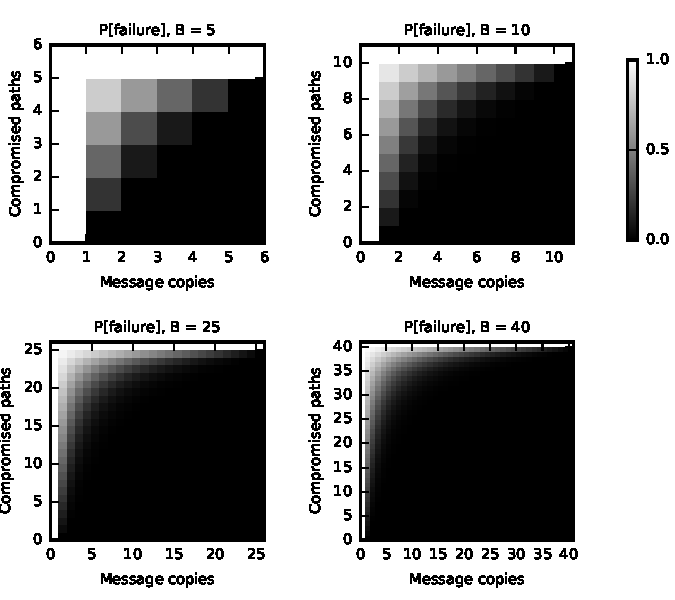
\includegraphics{fig-perror}}
\caption{TODO}
\label{fig:one}
\end{figure}

\section{Multipath Routing on the Butterfly Topology}

\subsection{Butterfly Network Topology}

We now describe a Concurrent Multipath Routing scheme on a specific family
of networks: the butterfly network \cite{}.
Several variations on the butterfly network exist.
Specifically, we utilize the wrap-around butterfly.
We denote the $m$-dimensional directed wrap-around butterfly as $\wbf(m)$:
\beq
\wbf(m) &=& (V, E_\downarrow \cup E_\rightarrow) \\
V &=& \mathbb{Z}_m \times \mathbb{Z}_{2^m} \\
E_\downarrow &=& \{((l,z),(l+1 (\text{mod } m),z) \nonumber \\
&& \; | \, l \in \mathbb{Z}_d, z \in \mathbb{Z}_{2^m}\} \\
E_\rightarrow &=& \{(l,z),(l+1 (\text{mod } m), z \oplus 2^l) \nonumber \\
&& \; | \, l \in \mathbb{Z}_d, z \in \mathbb{Z}_{2^m}\},
\eeq
where $\oplus$ represents the bitwise XOR operator.
Each node is associated with a level $l$ and an $m$-bit integer $z$.
There are two types of edges, shown in Figure \ref{fig:butterfly}.
Down edges ($E_\downarrow$) connect nodes sharing the same $z$ value
in a cycle of increasing level $l$.
Down-right edges ($E_\rightarrow$) also link to a node of level $l + 1$,
but one having the bitstring equal to $z$ with the $l$th bit flipped.

The wrap-around butterfly network has a number of properties making it useful for multipath routing:
\begin{description}
\item[Vertex transitivity]
The problem
of finding a route between arbitrary nodes $v$ and $w$
can be reduced to finding a route from node $(0,0)$ to some $\tilde{w}$.
\item[Logarithmic diameter]
For any two nodes, the length of the shortest path between them is logarithmic
in the size of the network.
\item[Constant degree]
In practical applications, each communication link requires additional resources,
such as physical infrastructure or entries in a routing table.
A constant degree limits the number of such resources needed as the network
grows in size.
\item [Redundancy] 
As we show in the next section. The number of independent paths between two nodes increases exponentially with the size of the trusted neighborhood. 
\end{description}

\begin{figure}
\begin{center}
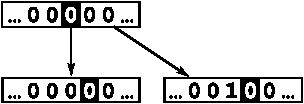
\includegraphics{fig-butterfly.pdf}
\end{center}
\caption{
Schematic illustration of the two types of edges in a directed butterfly network.
The node $(l,z)$ is shown as the bit string $z$ with a square around the $l$th bit.
\label{fig:butterfly}
}
\end{figure}

\subsection{Routing Algorithm: Overview}

This section gives an informal overview of the multipath routing algorithm.
In a wraparound butterfly network with trusted radius $h$,
the algorithm constructs $2^h$ disjoint paths between the trusted neighborhoods
of any two nodes $v$ and $w$. Because of vertex transitivity, we can make the simplifying assumption that $v = (0,0)$ without loss of generality. Each path is parameterized by an $h$-bit string $s \in (0,2^h]$ (see Table \ref{tab:routing}). Each path cycles around the levels of the butterfly network at most twice.


During the first cycle, the place-within-level $z$ of all nodes is set such that
no two paths overlap outside the trusted neighborhoods.
During the second cycle, the place-within-level is set to its destination value
and the algorithm terminates when the destination level is reached.

More specifically, consider any node, $(l,z)$, in the path corresponding to $s$. The algorithm can be understood by dividing the $m$ bits of
$z$ into four segments: $A, B, C, D$ (see figure \ref{fig:route-overview}).
$A$ is the first $h$ bits, followed by $B$ until reaching $C$, which is the last $h$ bits before
the destination level $l_w$, and then finally $D$. Hence, $A, B, C, $ and $D$ occupy $h$, $l_w - 2h$, $h$, and $m - l_w$ bits of $z$, respectively. 
Note that due to the construction of the network, as we walk through any path $\{p_1, p_2, \dots\}$, the level $l_{t+1}$ of node $p_{t+1}$ is always one higher (mod $m$) than level $l_t$ the previous node $p_t$. Also, $z_{t+1}$ is always the same as the $z_t$, except for possibly the $(l+1)^{th}$ bit of $z_{t+1}$, which can be either 0 or 1. Hence, as the routing algorithm progresses through the levels $l$, the segments of $z$ get updated in order. 

There are 7 stages of the algorithm to construct a path from $v$ to $w$. Stages (1) through (4) consist of the first cycle thought the levels of the network and stages (5) though (7) consists of the second (potentially partial) cycle. We start at the source node $v$ and begin constructing the path. During stage (1), $A$ is set to match $s$. During stage (2) the bits of $B$ are inverted. During stage (3) a cyclic permutation of $s$ is placed into $C$. After this, in stages (4--7), $D$, $A$, $B$, and $C$ are set to their destination values (see figure \ref{fig:route-overview}).

We now argue that in the above routing algorithm, given $s, s' \in (0, 2^h]$ such that $s \neq s'$, the corresponding paths, $P_s$ and $P_{s'}$, are disjoint when they are both outside of the trusted neighborhoods of $v$ and $w$. We informally refer to different segments of nodes in $s$ and $s'$ as $A,B,C,D$ and $A',B',C',D'$, respectively. 

First note that any over lap between the two paths must occur either while they are at the same stage of the routing, or while one is at stage (1) and the other one at (5), one is at stage (2) and the other one at (6), or one is at stage (3) and the other one at (7). This is because in any other case, the nodes in the paths will be at different levels, $l$, and thus they cannot overlap. Furthermore, when a path is in stage (1) or (7), it is in the trusted neighborhoods of $v$ or $w$, hence we are not concerned with overlaps in stages (1) or (7). 

When both paths are in stages (2), (3), or (4), they do not overlap because segment $A$ is set to $s$ and segment $A'$ is set to $s'$. When both paths are in stages (5) or (6), they do not overlap because segment $C$ is set to a cyclic permutation of $s$ and segment $C'$ is set to a cyclic permutation of $s'$. When one path is in stage (1) and the other one is in stage (5), say $P_s$ is in (1) and $P_{s'}$ is in (5), they do not overlap because all bits in $B$ are set to the original bits in the source node and all bits in $B'$ is set to the inverted bits of the source node. When one path is in stage (2) and the other one is in stage (6), they do not overlap because at least one pair of bits in $B$ and $B'$ is still be mismatched while stage (6) is being processed. 

\begin{figure}
\begin{center}
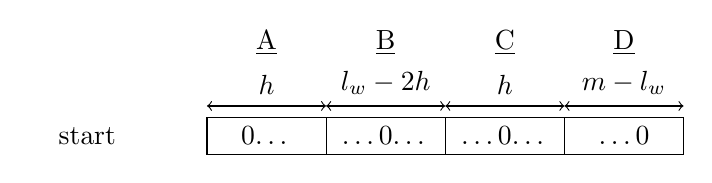
\begin{tikzpicture}[
node distance=0pt,
 start chain = A going right,
    X/.style = {rectangle, draw,% styles of nodes in string (chain)
                minimum width=10ex, minimum height=3ex,
                outer sep=0pt, on chain},
                        ]
\foreach \i in {0\ldots,{\ldots}0\ldots,{\ldots}0\ldots,{\ldots}0}% <-- content of nodes
    \node[X] {\i};
\draw[<->] ([yshift=1.5mm] A-1.north east) -- node[above=0.25mm] {$h$} ([yshift=1.5mm] A-1.north west);
\draw[<->] ([yshift=1.5mm] A-2.north east) -- node[above=0.25mm] {$l_w - 2h$} ([yshift=1.5mm] A-2.north west);
\draw[<->] ([yshift=1.5mm] A-3.north east) -- node[above=0.25mm] {$h$} ([yshift=1.5mm] A-3.north west);
\draw[<->] ([yshift=1.5mm] A-4.north east) -- node[above=0.25mm] {$m - l_w$} ([yshift=1.5mm] A-4.north west);
\draw ( A-1.west) -- node[left=5ex,minimum width=10ex] {start} ( A-1.west);
\node (B1) [inner sep=1pt,above=of A-1.north,above=5ex] {\underline{A}};
\node (B2) [inner sep=1pt,above=of A-2.north,above=5ex] {\underline{B}};
\node (B3) [inner sep=1pt,above=of A-3.north,above=5ex] {\underline{C}};
\node (B4) [inner sep=1pt,above=of A-4.north,above=5ex] {\underline{D}};
\end{tikzpicture}
\\
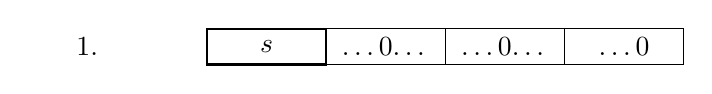
\begin{tikzpicture}[
node distance=0pt,
 start chain = A going right,
    X/.style = {rectangle, draw,% styles of nodes in string (chain)
                minimum width=10ex, minimum height=3ex,
                outer sep=0pt, on chain},
    Y/.style = {rectangle, draw,% styles of nodes in string (chain)
                minimum width=10ex, minimum height=3ex,
                outer sep=0pt, on chain, thick},
                        ]
\node[Y] {$s$};
\foreach \i in {{\ldots}0\ldots,{\ldots}0\ldots,{\ldots}0}% <-- content of nodes
    \node[X] {\i};
\draw ( A-1.west) -- node[left=5ex,minimum width=10ex] {1.} ( A-1.west);
\end{tikzpicture}
\\
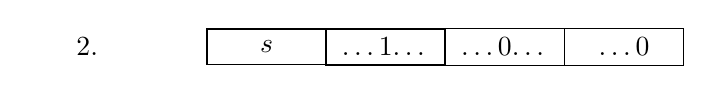
\begin{tikzpicture}[
node distance=0pt,
 start chain = A going right,
    X/.style = {rectangle, draw,% styles of nodes in string (chain)
                minimum width=10ex, minimum height=3ex,
                outer sep=0pt, on chain},
    Y/.style = {rectangle, draw,% styles of nodes in string (chain)
                minimum width=10ex, minimum height=3ex,
                outer sep=0pt, on chain, thick},
                        ]
\foreach \i in {$s$}% <-- content of nodes
    \node[X] {\i};
\node[Y] {{\ldots}1\ldots};
\foreach \i in {{\ldots}0\ldots,{\ldots}0}% <-- content of nodes
    \node[X] {\i};
\draw ( A-1.west) -- node[left=5ex,minimum width=10ex] {2.} ( A-1.west);
\end{tikzpicture}
\\
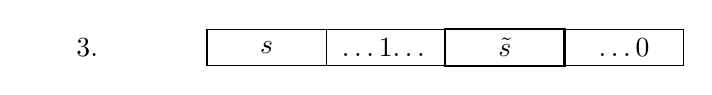
\begin{tikzpicture}[
node distance=0pt,
 start chain = A going right,
    X/.style = {rectangle, draw,% styles of nodes in string (chain)
                minimum width=10ex, minimum height=3ex,
                outer sep=0pt, on chain},
    Y/.style = {rectangle, draw,% styles of nodes in string (chain)
                minimum width=10ex, minimum height=3ex,
                outer sep=0pt, on chain, thick},
                        ]
\foreach \i in {$s$,{\ldots}1\ldots}% <-- content of nodes
    \node[X] {\i};
\node[Y] {$\tilde{s}$};
\foreach \i in {{\ldots}0}% <-- content of nodes
    \node[X] {\i};
\draw ( A-1.west) -- node[left=5ex,minimum width=10ex] {3.} ( A-1.west);
\end{tikzpicture}
\\
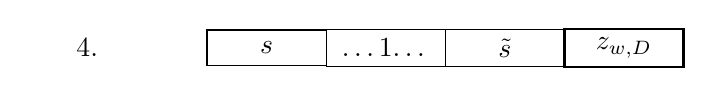
\begin{tikzpicture}[
node distance=0pt,
 start chain = A going right,
    X/.style = {anchor=base, rectangle, draw,% styles of nodes in string (chain)
                minimum width=10ex, minimum height=3ex,
                outer sep=0pt, on chain},
    Y/.style = {rectangle, draw,% styles of nodes in string (chain)
                minimum width=10ex, minimum height=3ex,
                outer sep=0pt, on chain, thick},
                        ]
\foreach \i in {$s$,{\ldots}1\ldots,$\tilde{s}$}% <-- content of nodes
    \node[X] {\i};
\node[Y] {$z_{w,D}$};
\draw ( A-1.west) -- node[left=5ex,minimum width=10ex] {4.} ( A-1.west);
\end{tikzpicture}
\\
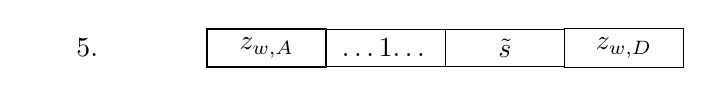
\begin{tikzpicture}[
node distance=0pt,
 start chain = A going right,
    X/.style = {anchor=base, rectangle, draw,% styles of nodes in string (chain)
                minimum width=10ex, minimum height=3ex,
                outer sep=0pt, on chain},
    Y/.style = {rectangle, draw,% styles of nodes in string (chain)
                minimum width=10ex, minimum height=3ex,
                outer sep=0pt, on chain, thick},
                        ]
\node[Y] {$z_{w,A}$};
\foreach \i in {{\ldots}1\ldots,$\tilde{s}$,$z_{w,D}$}% <-- content of nodes
    \node[X] {\i};
\draw ( A-1.west) -- node[left=5ex,minimum width=10ex] {5.} ( A-1.west);
\end{tikzpicture}
\\
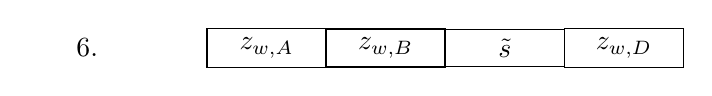
\begin{tikzpicture}[
node distance=0pt,
 start chain = A going right,
    X/.style = {anchor=base, rectangle, draw,% styles of nodes in string (chain)
                minimum width=10ex, minimum height=3ex,
                outer sep=0pt, on chain},
    Y/.style = {rectangle, draw,% styles of nodes in string (chain)
                minimum width=10ex, minimum height=3ex,
                outer sep=0pt, on chain, thick},
                        ]
\foreach \i in {$z_{w,A}$}% <-- content of nodes
    \node[X] {\i};
\node[Y] {$z_{w,B}$};
\foreach \i in {$\tilde{s}$,$z_{w,D}$}% <-- content of nodes
    \node[X] {\i};
\draw ( A-1.west) -- node[left=5ex,minimum width=10ex] {6.} ( A-1.west);
\end{tikzpicture}
\\
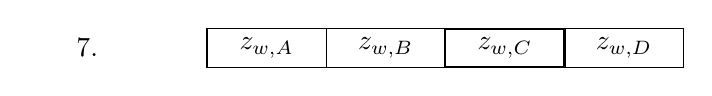
\begin{tikzpicture}[
node distance=0pt,
 start chain = A going right,
    X/.style = {anchor=base, rectangle, draw,% styles of nodes in string (chain)
                minimum width=10ex, minimum height=3ex,
                outer sep=0pt, on chain},
    Y/.style = {rectangle, draw,% styles of nodes in string (chain)
                minimum width=10ex, minimum height=3ex,
                outer sep=0pt, on chain, thick},
                        ]
\foreach \i in {$z_{w,A}$,$z_{w,B}$}% <-- content of nodes
    \node[X] {\i};
\node[Y] {$z_{w,C}$};
\foreach \i in {$z_{w,D}$}% <-- content of nodes
    \node[X] {\i};
\draw ( A-1.west) -- node[left=5ex,minimum width=10ex] {7.} ( A-1.west);
\end{tikzpicture}
\end{center}
\caption{
Progression of place-within-level $z$ as the multipath routing algorithm
cycles through the levels of the butterfly network.
}
\label{fig:route-overview}
\end{figure}

\begin{table}%
\tbl{Butterfly Multipath Routing Variables\label{tab:routing}}
{
\begin{tabular}{|l|l|}
\hline
NAME & VARIABLE \\\hline
butterfly dimension & $m \in \mathbb{Z}_+$ \\\hline
node level & $l \in \mathbb{Z} : 0 \leq l < m$ \\\hline
node place within level & $z \in \mathbb \{0,1\}^m$ \\\hline
trust radius & $h \in \mathbb{Z} : 1 \leq h \leq \lfloor m/2 \rfloor$ \\\hline
path index & $s \in \{0,1\}^h$ \\\hline
\end{tabular}
}
\end{table}%

\subsection{Routing Algorithm: Proof}

We now describe a routing scheme that provides $2^h$ redundant paths between
the $h$-hop trusted neighborhoods of any two nodes in an $m$-bit
wrap-around butterfly network.
Utilizing vertex transitivity, we label the source node as $(0, 0)$ and
denote the destination node as $w = (l_w, z_w)$.

Let $s$ be an integer such that $0 \leq s < 2^h$.
Let $v_s^{(t)} = (l^{(t)}, z^{(t)})$ be the $t$th node in the path labeled by $s$.
For convenience, we will omit the subscript $s$.
We define two partitionings of the integers in $\mathbb{Z}_{2^m}$:
one having the lowest $h$ bits matching the
bits of $s$, and one having the $h$ bits preceeding the destination level $l_w$
matching $s$:
\beq
S_s &=& \{z \in \mathbb{Z}_{2^m} | \forall i \in \mathbb{Z}_h z_i = s_i \} \\
R_s &=& \{z \in \mathbb{Z}_{2^m} | \forall i \in \mathbb{Z}_h z_{(l_w - h + i)} = s_i \}.
\eeq
Note that if $r \neq s$, then $S_s \cap S_r = R_s \cap R_r = \emptyset$.

We now construct a path such that between trusted neighborhoods $z^{(t)}$ is always
in $S_s$, $R_s$, or both, guaranteeing that the path does not overlap with the
other paths $v_r^{(t)}$.
Routing proceeds in stages, with the level $l$ increasing by 1 at each hop.
In Stage 1 ($0 \leq t < h$), down or down-right edges
are chosen such that the $t$th bit of $z^{(t+1)}$ is equal to the $t$th bit
of $s$. Throughout Stage 1, all nodes are within the sender's trusted neighborhood.
At the end of Stage 1, $z^{(h)} \in S_s$, and $z^{(t)}$ will remain so until the level loops
back to $0$ at $t = m$.

In Stage 2 ($h \leq t < l_w - h$), edges are chosen to make the $t$th bit of
$z^{(t+1)}$ match the $t$th bit of $z_w$.

In Stage 3 ($l_w - h \leq t < l_w$), the bits of $z^{(t)}$ are chosen to match $s$,
such that after the stage is complete, $z^{(l_w)} \in R_s$.

In Stage 4 ($l_w \leq t < m$), as in stage 2,
paths are chosen such that the $t$th bit of $z^{(t+1)}$ matches $z_w$.
After Stage 4, all bits of $z^{(m)}$ are equal to those of $z_w$
except for the first $h$ and the $h$ preceeding index $l_w$.
$z^{(m)}$ is also in both $S_s$ and $R_s$.

At this point, we define $\tau = t - m$.
In Stage 5 ($0 \leq \tau < h$), the first $h$ bits of $z^{(t)}$ are set to
match $z_w$, potentially removing $z^{(t)}$ from $S_s$.

In Stage 6 ($h \leq \tau < l_w - h$), all down edges are chosen, incrementing
the level without any effect on $z^{(t)}$.
At the end of Stage 6, $z^{(m + l_w - h)}$ is still in $R_s$ and
$v^{(m + l_w - h)}$ is now within the trusted neighborhood of $w$.

In the seventh, and final stage ($l_w - h \leq \tau < l_w$), the $h$ bits of $z^{(t)}$
preceeding index $l_w$ are set to match $z_w$.
After this stage, $v^{(m + l_w)} = w$ and routing is complete.

\begin{figure}
\begin{center}
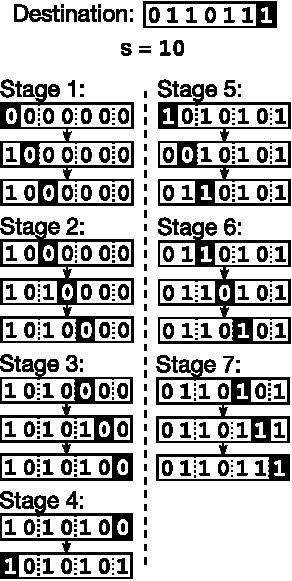
\includegraphics{fig-routing.pdf}
\end{center}
\caption{
\label{fig:routing}
}
\end{figure}

\section{Discussion}

Secrecy

Creation of the network.
Improves on web of trust.
Gives framework for determining where to build trust.

Applications
Distributed apps: storage, email, cryptocurrency, secure multiparty computation.
Wireless Sensor Networks

\section{Conclusion}

% Acknowledgments
\begin{acks}
The authors would like to thank TODO
\end{acks}

% Bibliography
\bibliographystyle{ACM-Reference-Format-Journals}
\bibliography{paper}

\end{document}
